\documentclass[a4paper]{article}

\usepackage[polish]{babel}
	\addto{\captionspolish}{\renewcommand{\abstractname}{}}
\usepackage[OT4]{polski}
\usepackage[utf8]{inputenc}
\usepackage{amsmath}
\usepackage{graphicx}
\usepackage[colorinlistoftodos]{todonotes}
\usepackage[top = 3cm, bottom = 4cm, left = 2cm, right = 2cm]{geometry}
\usepackage{indentfirst}
\usepackage{caption}
\usepackage{subcaption}
\usepackage[nodayofweek,level]{datetime}

\usepackage{placeins}		% for FloatBarriers
\usepackage{float}
\usepackage{booktabs}
\usepackage{array}
\newcolumntype{L}[1]{>{\raggedright\let\newline\\\arraybackslash\hspace{0pt}}m{#1}}
\newcolumntype{C}[1]{>{\centering\let\newline\\\arraybackslash\hspace{0pt}}m{#1}}
\newcolumntype{R}[1]{>{\raggedleft\let\newline\\\arraybackslash\hspace{0pt}}m{#1}}

\newcounter{rownum}	%table counter
	\newcommand\rownum{\stepcounter{rownum}\arabic{rownum}}
\setcounter{rownum}{0}

\usepackage[framed,numbered,autolinebreaks,useliterate]{mcode}


\title{Filtracja sygnałów metodą Savitzky'ego-Golaya \\ Raport cząstkowy}

\author{Klaudia Luks, Wojciech Karkoszka}

\date{\formatdate{22}{12}{2016}}

\begin{document}
\maketitle
%%%%%%%%%%%%%%%%%%%%%%%%%%%%%%%%%%%%%%%%%%%%%%%%%%%%%%%%%%%%%%%%%%%%%%%%%%%%%%%%%%%%%%%%%%%%%%%%%%%

\section{Wstęp}

W niniejszym raporcie przedstawiona została prototypowa implementacja filtru Savitzky'ego-Golaya na potrzeby analizy sygnału elektrokardiograficznego. Algorytm został zbudowany i przetestowany w oparciu o sygnały pochodzące z bazy MIT-BIH, a otrzymane wyniki przedstawione zostały w dalszej części raportu.

%%%%%%%%%%%%%%%%%%%%%%%%%%%%%%%%%%%%%%%%%%%%%%%%%%%%%%%%%%%%%%%%%%%%%%%%%%%%%%%%%%%%%%%%%%%%%%%%%%%

\section{Filtracja Savitzky'ego Golaya}

Filtracja Savitzky'ego-Golaya polega na wygładzaniu danych wejściowych za pomocą aproksymacji wielomianu metodą najmniejszych kwadratów. Lokalne dopasowywanie wielomianów i obliczanie wartości wielomianu dla środkowego punktu analizowanego interwału jest równoważne działaniu na sygnał odpowiednim filtrem \cite{on}. Przesuwając okno, w którym następuje dopasowanie odpowiedniej krzywej, uzyskuje się -- dla środkowej próbki przedziału -- wartość wygładzoną. Filtry Savitzky'ego-Golaya mona traktować jak filtry o skończonej odpowiedzi impulsowej (FIR). Szczególnym przypadkiem tego rodzaju filtracji jest filtr ruchomej średniej (w przypadku, gdy rząd wielomianu aproksymacyjnego wynosi 0).

Co istotne, wygładzanie zaszumionego sygnału tą metodą zwiększa stosunek sygnału do szumu, ale jednocześnie dość dobrze zachowuje kształt i amplitudę poszczególnych pików \cite{what}. Ta własność znajduje szczególne zastosowanie w sygnałach elekardiograficznych \cite{what}, gdzie na podstawie morfologii zespołów QRS można rozpoznać wiele zaburzeń, tak więc sygnał przefiltrowany musi być jak najmniej zniekształcony. Algorytm może jednak powodować niekorzystne efekty brzegowe, które mogą zostać uniknięte poprzez nadbudowanie sygnału wejściowego na brzegach o określoną liczbę próbek.

Zalety filtracji Savitzky'ego-Golaya to tendencja do zachowywania wysokości i szerokości szczytów oryginalnego sygnału, płaska charakterystyka w zakresie pasma przepustowego i liniowe przesunięcie fazowe. Do wad algorytmu można zaliczyć pojawienie się efektów brzegowych na końcach sygnału (czemu można jednak zaradzić rozszerzając odpowiednio sygnał) oraz konieczność obliczania współczynników wielomianu dla każdorazowo przesuniętego okna, co wiąże się z kosztowną obliczeniowo operacją odwracania macierzy \cite{per-olof}.

%%%%%%%%%%%%%%%%%%%%%%%%%%%%%%%%%%%%%%%%%%%%%%%%%%%%%%%%%%%%%%%%%%%%%%%%%%%%%%%%%%%%%%%%%%%%%%%%%%%

\section{Opis algorytmu}

\subsection {Opis matematyczny}

Zadaniem algorytmu jest dopasowanie w kolejnych fragmentach sygnału wielomianu, który najlepiej przybliża otrzymane dane. Wynaczanie współczynników takiego wielomianu może zostać oparte o metodę najmniejszych kwadratów \cite{least-squares} -- należy znaleźć takie, które minimalizują wartość funkcji:

\begin{equation} \label{eq1}
S(a_0, ..., a_K) = \sum_{i=1}^N \left( y_i - y(x_i) \right)^2
\end{equation}

gdzie K -- rząd dopasowywanego wielomianu, $(x_i, y_i)$ -- punkty poddawane filtracji, $y$ -- funkcja opisująca dopasowany wielomian.\\

Aby znaleźć minimum takiej funkcji możemy znaleźć miejsca, w których pochodne cząstkowe funkcji są równe zeru. Oznacza to rozwiązanie układu równań składającego się z wyrażeń dla każdej k-tej wartości współczynnika:

\begin{equation}
\frac{\delta S(a_0, ..., a_K)}{\delta a_k} = 0
\end{equation}

Zatem:

\begin{equation}
\frac{\delta}{\delta a_k} \sum_{i=1}^N \left( y_i - y(x_i) \right)^2 = 0
\end{equation}

\begin{equation}
\frac{\delta}{\delta a_k}\sum_{i=1}^N \left( y_i - \left(a _0 + ... + a_K x_i^K \right)\right)^2 = 0
\end{equation}

\begin{equation}
2\sum_{i=1}^N \left( y_i - a_0 - ... - a_K x_i^K \right) (- x_i^k) = 0
\end{equation}

Stąd otrzymać możemy układ równań o wyrazach w postaci:

\begin{equation}
\sum_{j=0}^K a_j \sum_{i=1}^N x_i^{j+k} = \sum_{i=1}^N y_i x_i^k
\end{equation}

Co można przedstawić w postaci macierzowej:

\begin{equation} \label{matrices}
\begin{bmatrix}
    N      & \sum_{i=1}^N x_i & \dots & \sum_{i=1}^N x_i^{K} \\
    \sum_{i=1}^N x_i      & \sum_{i=1}^N x_i^2 & \dots & \sum_{i=1}^N x_i^{K+1} \\
    \vdots & \vdots & \ddots & \vdots \\
\sum_{i=1}^N x_i^K      & \sum_{i=1}^N x_i^{1+K} & \dots & \sum_{i=1}^N x_i^{2K}\\
\end{bmatrix}
\begin{bmatrix}
    a_0	\\
    a_1	\\
    \vdots	\\
    a_N
\end{bmatrix}
=
\begin{bmatrix}
    \sum_{i=1}^N y_i	\\
    \sum_{i=1}^N y_i x_i	\\
    \vdots	\\
    \sum_{i=1}^N y_i x_i^K
\end{bmatrix}
\end{equation}

Mnożąc lewostronnie przez odwrotność pierwszej z macierzy otrzymujemy wartości współczynników:

\begin{equation}
(X^{-1}) X A = X^{-1}Y
\end{equation}

\begin{equation}
A = X^{-1}Y
\end{equation}

Kolejnym krokiem jest obliczenie wartości dopasowanego wielomianu dla jednej z próbek znajdującej się w oknie -- w naszym przypadku jest to środek okna.


\begin{equation}
y_{filtered} = \sum_{i=1}^K a_k x_i^k
\end{equation}




\subsection {Opis implementacyjny}

Schemat blokowy algorytmu realizującego filtrację Savitzky'ego-Golaya został przedstawiony na rys. \ref{uml}. 

\begin{figure}[H]
\centering
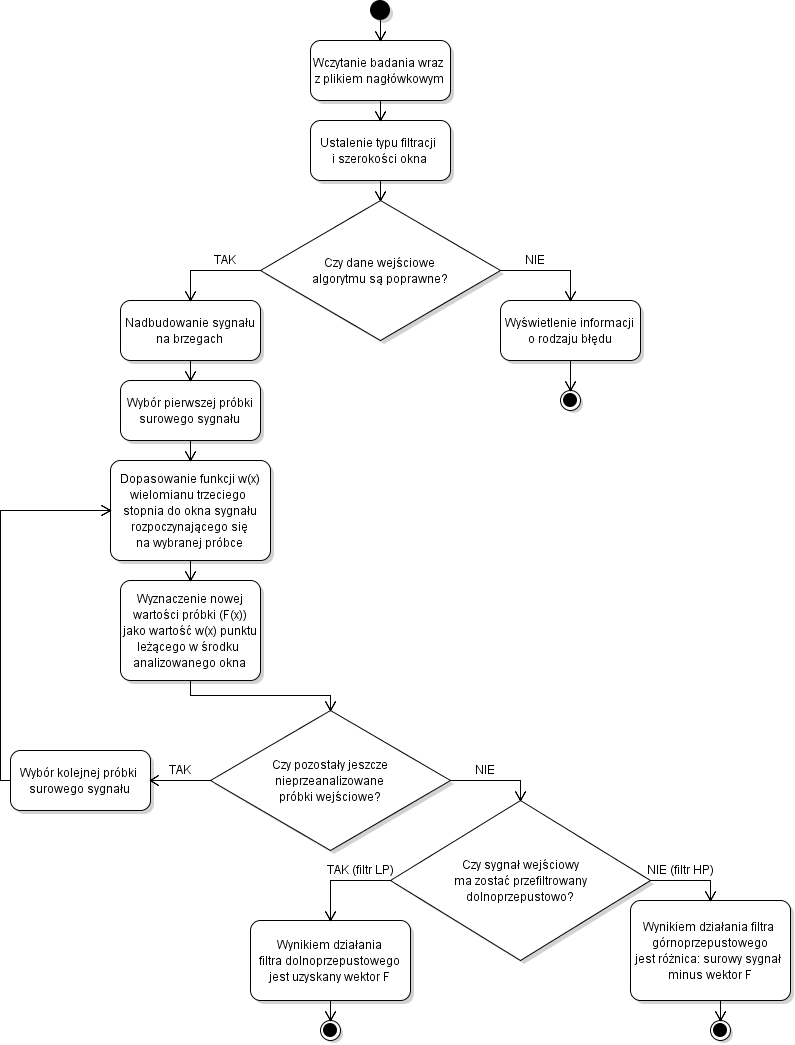
\includegraphics[width=1\textwidth]{algorytm_uml.png}
\caption{\label{uml} Diagram UML przedstawiający działanie zaimplementowanego algorytmu filtracji Savitzky'ego - Golaya.}
\end{figure}

Na początku sprawdzana jest poprawność danych wejściowych, między innymi:
\begin{itemize}
\item Czy sygnał wejściowy jest niepustą tablicą?
\item Czy sygnał wejściowy składa się z dwóch kanałów? (specyfika bazy MIT-BIH)
\item Czy zmienna określająca typ filtra ma wyłącznie wartość 1 (filtr dolnoprzepustowy) lub 2 (filtr górnoprzepustowy)?
\item Czy szerokość okna filtracji jest liczbą całkowitą dodatnią?
\item Czy szerokość okna jest liczbą nieparzystą? Jest to konieczne, ponieważ w każdej iteracji algorytmu wybierana jest środkowa próbka okna. Jeżeli szerokość okna jest liczbą parzystą, następuje jej inkrementacja o 1.
\end{itemize}

W następnej kolejności surowy sygnał jest poszerzany zarówno na początku, jak i na końcu o liczbę próbek równą całkowitoliczbowej połowie szerokości okna.

Następnie iterując po surowym sygnale tworzone są okna, do których dopasowywany jest wielomian trzeciego stopnia. Wartość przybliżonego wielomianu w samym środku okna jest uznawana za próbkę wyjściową danej iteracji, co jest widoczne we fragmencie kodu poniżej (listing \ref{polyfit}).


\begin{lstlisting}[caption=Fragment algorytmu realizujący dopasowanie wielomianu trzeciego stopnia i obliczenie wartości wyjściowej danej próbki jako wartość funkcji wielomianowej w środku okna rozpoczynającego się w tej próbce., label=polyfit]
    bnd = floor(window_width / 2);
    
	% ... 
    
    for i=1:length(raw_signal)

        % interpolation coefficients       
        coeffs = polyfit((i:i+window_width-1)', ...
            expanded_sig(i:i+window_width-1), 3);

        % output signal for every sample        
        filtered_signal(i) = coeffs(1) * (i+bnd)^3 + ...
            coeffs(2) * (i+bnd) ^2 + ...
            coeffs(3) * (i+bnd) + coeffs(4);
    end
\end{lstlisting}

Algorytm jest dostosowany zarówno do filtracji dolno-, jak i górnoprzepustowej, a różnica polega jedynie na wykonywaniu bądź nie operacji odjęcia uzyskanego wektora od wektora surowego sygnału.

%%%%%%%%%%%%%%%%%%%%%%%%%%%%%%%%%%%%%%%%%%%%%%%%%%%%%%%%%%%%%%%%%%%%%%%%%%%%%%%%%%%%%%%%%%%%%%%%%%%

\section{Rezultaty}

Na rysunkach \ref{filt1}, \ref{filt2}, \ref{filt1_109}, \ref{filt2_109} przedstawiono zastosowanie filtru w praktyce na fragmentach badania z bazy nagrań MIT-BIH. Sygnały najpierw zostały poddane filtracji dolnoprzepustowej, a następnie wynikowy sygnał poddano filtracji górnoprzepustowej, co zostało oznaczone odpowiednimi kolorami. 

\textbf{Filtracja dolnoprzepustowa} zredukowała zakłócenia sygnału. W rezultacie widoczne jest, że oscylacje sygnału surowego ''wystają'' poza sygnał wygładzony po filtracji dolnoprzepustowej (rys. \ref{filt1}, \ref{filt2}, \ref{filt1_109}, \ref{filt2_109}). W filtracji dolnoprzepustowej przyjęto szerokość okna równą $11$ próbek.

\textbf{Filtracja górnoprzepustowa} wyrównała izolinię sygnału do poziomu zera i zlikwidowała pływającą izolinię (szczególnie dobrze widoczne jest to na rysunkach \ref{filt2}, \ref{filt1_109} i  \ref{filt2_109}). W filtracji górnoprzepustowej przyjęto szerokość okna równą $85$ próbek.

\begin{figure}[H]
\centering
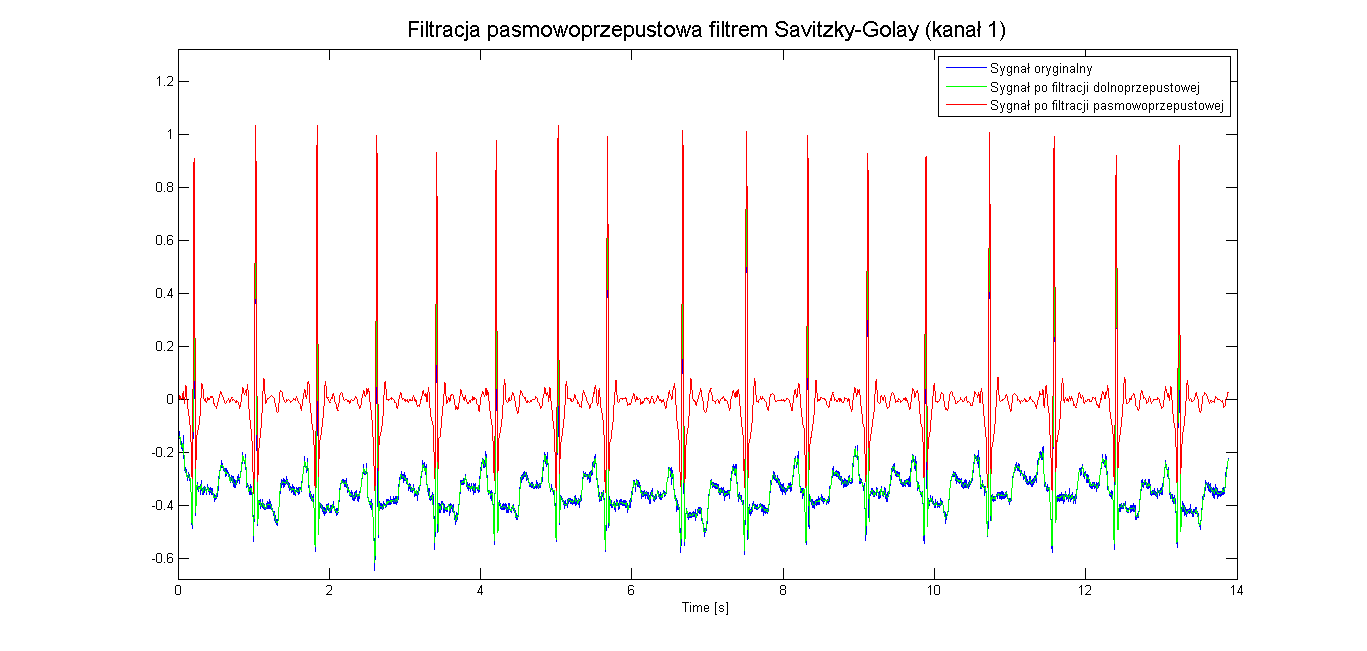
\includegraphics[width=1\textwidth]{100_filt1.png}
\caption{\label{filt1} Fragment sygnału \textit{'100.dat'}, odprowadzenie MLII, poddany filtracji pasmowoprzepustowej filtrami Savitzky\'ego - Golaya na poszczególnych etapach przetwarzania.}
\end{figure}

\begin{figure}[H]
\centering
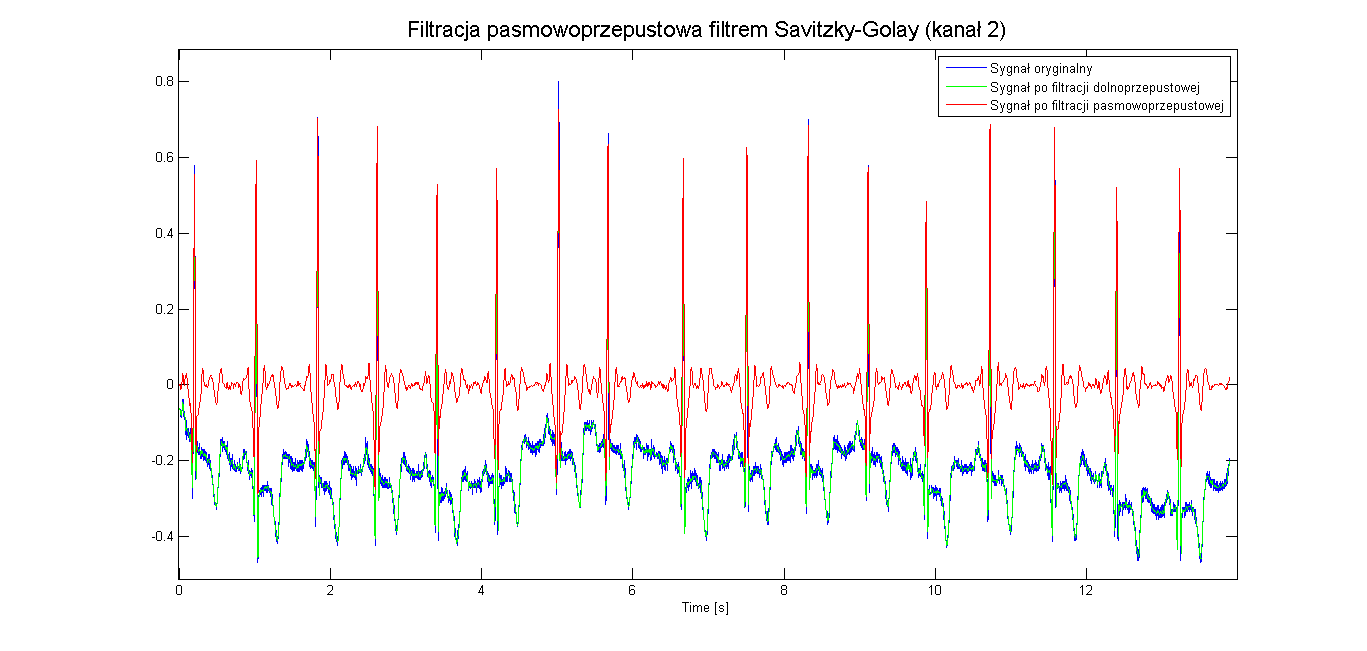
\includegraphics[width=1\textwidth]{100_filt2.png}
\caption{\label{filt2} Sygnał \textit{'100.dat'}, odprowadzenie V5, poddany filtracji pasmowoprzepustowej filtrami Savitzky\'ego - Golaya na poszczególnych etapach przetwarzania.}
\end{figure}

\begin{figure}[H]
\centering
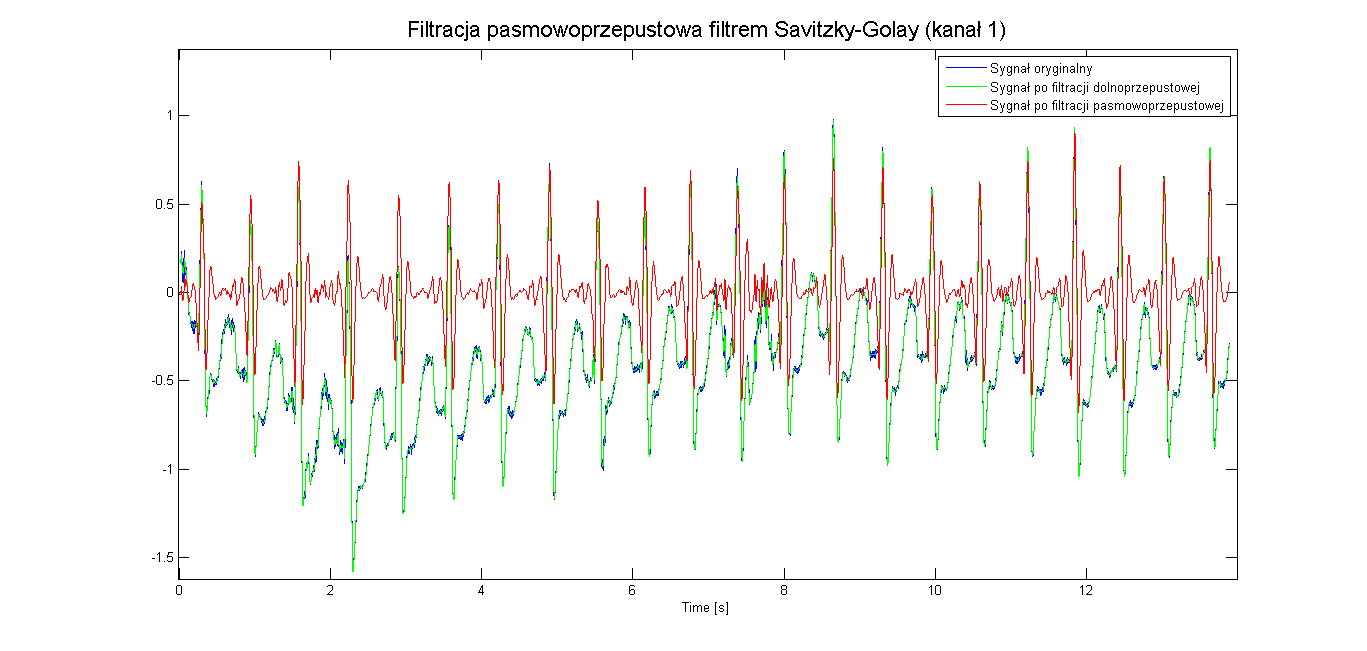
\includegraphics[width=1\textwidth]{109_filt1.png}
\caption{\label{filt1_109} Sygnał \textit{'109.dat'}, odprowadzenie MLII, poddany filtracji pasmowoprzepustowej filtrami Savitzky\'ego - Golaya na poszczególnych etapach przetwarzania.}
\end{figure}

\begin{figure}[H]
\centering
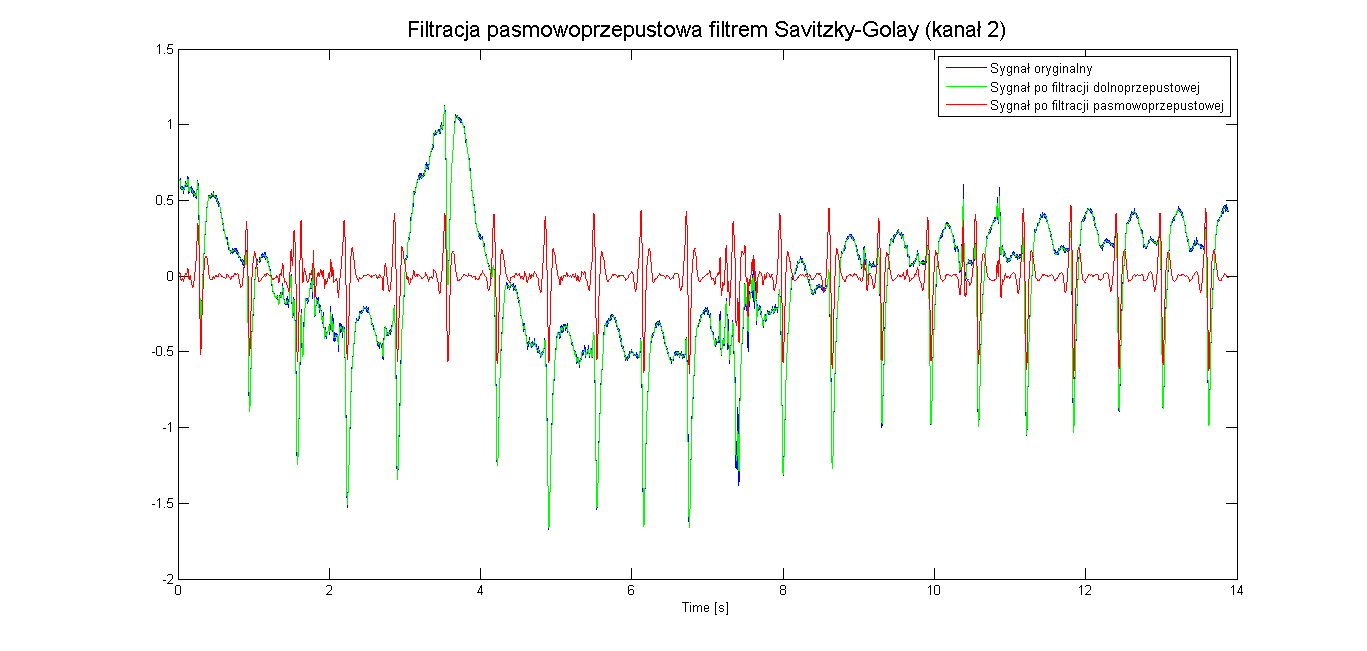
\includegraphics[width=1\textwidth]{109_filt2.png}
\caption{\label{filt2_109} Sygnał \textit{'109.dat'}, odprowadzenie V1, poddany filtracji pasmowoprzepustowej filtrami Savitzky\'ego - Golaya na poszczególnych etapach przetwarzania.}
\end{figure}

%%%%%%%%%%%%%%%%%%%%%%%%%%%%%%%%%%%%%%%%%%%%%%

\section{Podsumowanie}

W chwili obecnej działanie algorytmu filtracji Savitzky'ego - Golaya daje satysfakcjonujące efekty, jednak zajmuje dużo czasu, co utrudnia jego uruchomienie na większej ilości danych, w tym na całej bazie MIT-BIH.

W związku z tym dalszej części projektu uwaga zostanie skupiona na dwóch aspektach:
\begin{itemize}
\item implementacja tegoż algorytmu w języku C++ w celu zwiększenia jego wydajności;
\item przygotowanie systemu walidacji algorytmu w celu porównania wyników z innymi zespołami w ramach raportu zbiorczego.
\end{itemize}

%%%%%%%%%%%%%%%%%%%%%%%%%%%%%%%%%%%%%%%%%%%%%%%%%%%%%%%%%%%%%%%%%%%%%%%%%%%%%%%%%%%%%%%%%%%%%%%%%%%

%%%%%%%%%%%%%%%%%%%%%%%%%%%%%%%%%%%%%%%%%%%%%%%%%%%%%%%%%%%%%%%%%%%%%%%%%%%%%%%%%%%%%%%%%%%%%%%%%%%
\begin{thebibliography}{9}

\bibitem{on}
Krishnan S. R., Seelamantula C. S.\textit{On the Selection of Optimum Savitzky-Golay Filters}. IEEE transactions on signal processing 61.2 (2013): 380-391.

\bibitem{what}
Schafer R. W. \textit{What is a Savitzky-Golay filter?[lecture notes]}. IEEE Signal Processing Magazine 28.4 (2011): 111-117.

\bibitem{per-olof}
Persson, P., Strang, G. \textit{Smoothing by Savitzky-Golay and legendre filters}. Mathematical systems theory in biology, communications, computation, and finance (2003): 301-315.

\bibitem{least-squares}
Miller, S. J. \textit{The method of least squares}. Mathematics Department Brown University (2006): 1-7.

\end{thebibliography}


\pagebreak\newpage

\section*{Dodatek A: Kod źródłowy prototypów programu}

\lstinputlisting[caption=Wywołanie funkcji realizującej filtrację Savitzky'ego-Golaya., label=main]{multichannel_main.m}

\lstinputlisting[caption=Funkcja filtrująca dla wielu kanałów., label=s-g-foo]{sav_gol_multichannel.m}

\end{document}
